\chapter{QoS and Voice VLANs: Part 1}\label{qos-and-voice-vlans-part-1}

\section{IP Phones / Voice LANS}\label{ip-phones-voice-lans}

\begin{itemize}
\tightlist
\item
  Traditional phones operate over the \emph{public switched telephone
  network} (PSTN)

  \begin{itemize}
  \tightlist
  \item
    Sometimes, this is called POTS (Plain Old Telephone System)
  \end{itemize}
\item
  IP PHONES use VoIP (Voice Over IP) technologies to enable phone calls
  over an IP NETWORK, such as the INTERNET
\item
  IP PHONES are connected to a SWITCH, just like any other end HOST
\end{itemize}

\section{IP Phones}\label{ip-phones}

\begin{itemize}
\tightlist
\item
  Have an internal 3-PORT SWITCH

  \begin{itemize}
  \tightlist
  \item
    1 PORT is the ``UPLINK'' to the EXTERNAL SWITCH
  \item
    1 PORT is the ``DOWNLINK'' to the PC
  \item
    1 PORT connects internally to the PHONE itself
  \end{itemize}
\end{itemize}

\begin{figure}
\centering
\pandocbounded{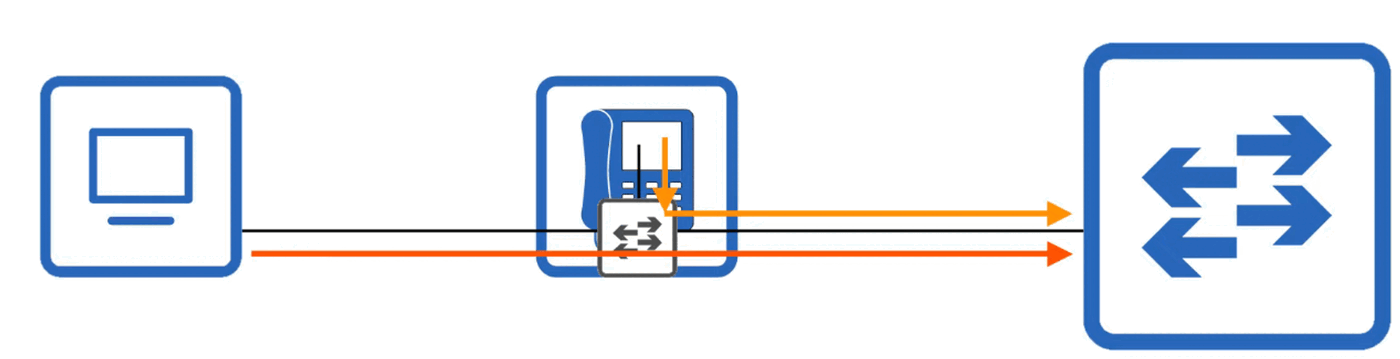
\includegraphics[keepaspectratio,alt={image}]{images/47-qos-voicelan/img-001.png}}
\end{figure}

\begin{itemize}
\tightlist
\item
  This allows the PC and the IP PHONE to share a single SWITCH PORT.
  Traffic from the PC passes through the IP PHONE to the SWITCH
\item
  It is RECOMMENDED to separate ``VOICE'' traffic (from IP PHONE) and
  ``DATA TRAFFIC'' (from the PC) by placing them into SEPARATE VLANS (!)

  \begin{itemize}
  \tightlist
  \item
    This can be accomplished using a VOICE VLAN
  \item
    Traffic from the PC will be UNTAGGED - but traffic from the PHONE
    will be tagged with a VLAN ID
  \end{itemize}
\end{itemize}

\begin{figure}
\centering
\pandocbounded{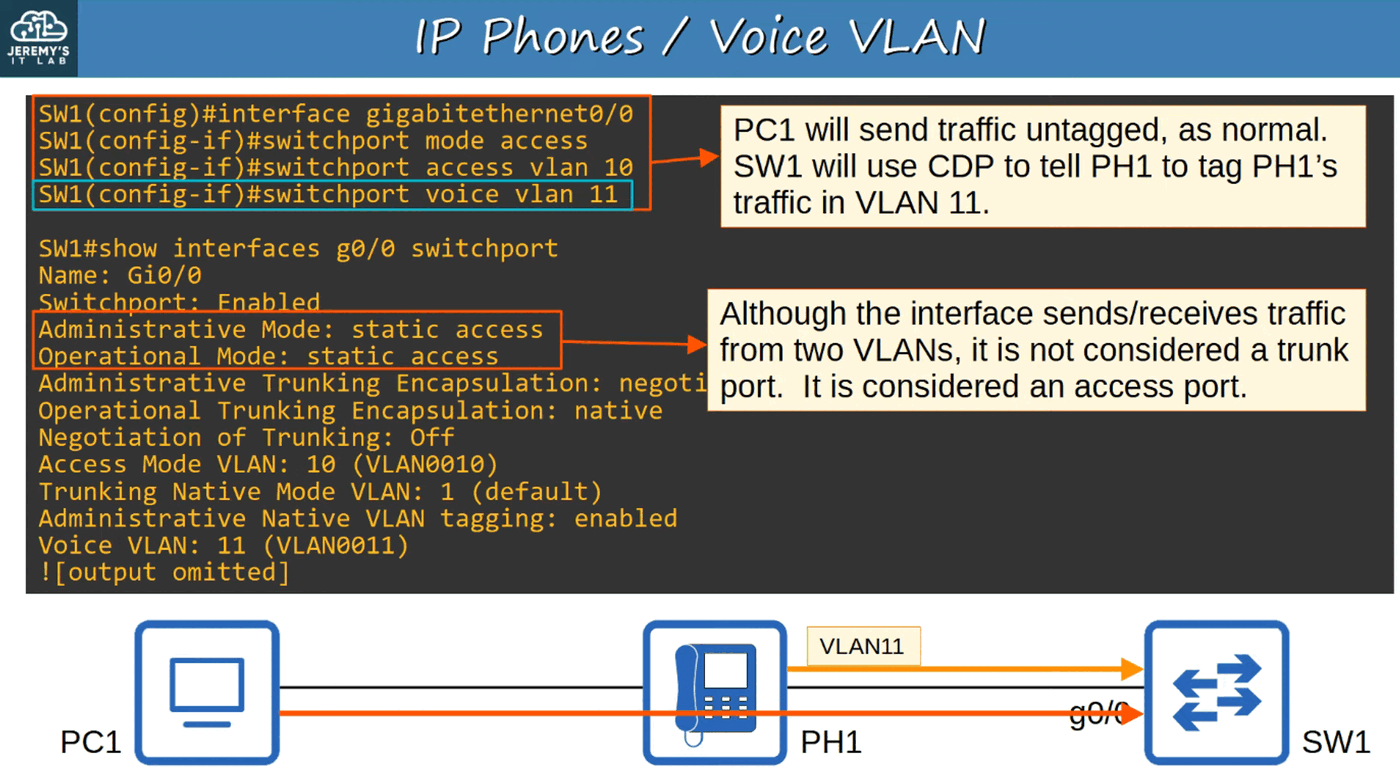
\includegraphics[keepaspectratio,alt={image}]{images/47-qos-voicelan/img-002.png}}
\end{figure}

\begin{figure}
\centering
\pandocbounded{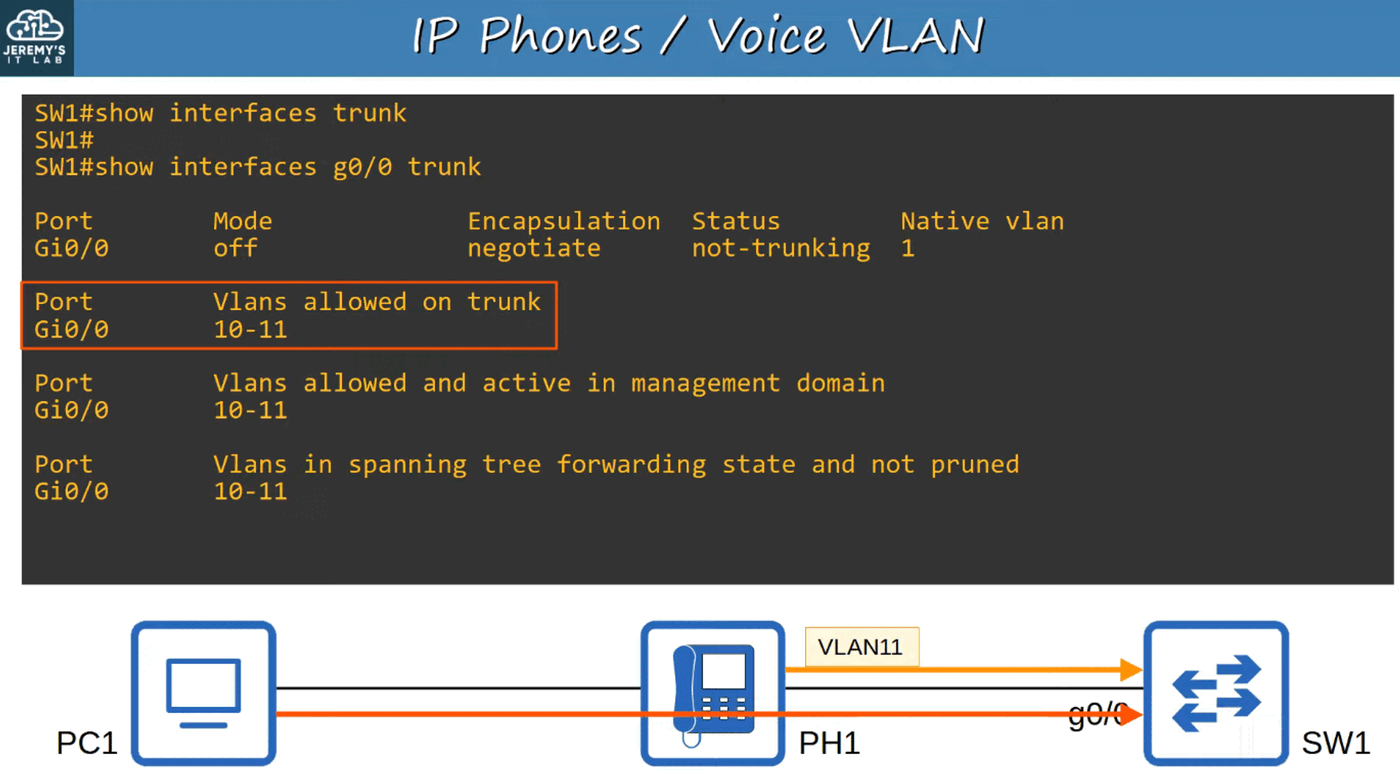
\includegraphics[keepaspectratio,alt={image}]{images/47-qos-voicelan/img-003.png}}
\end{figure}

\begin{figure}
\centering
\pandocbounded{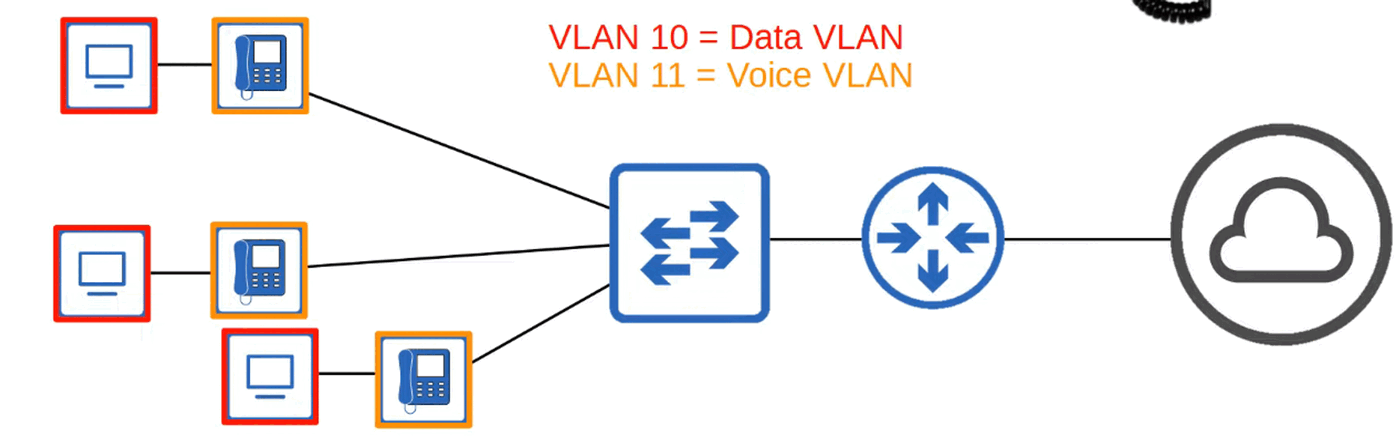
\includegraphics[keepaspectratio,alt={image}]{images/47-qos-voicelan/img-004.png}}
\end{figure}

POWER OVER ETHERNET (PoE)

\begin{itemize}
\tightlist
\item
  PoE allows Power Sourcing Equipment (PSE) to provide POWER to Powered
  Devices (PD) over an ETHERNET cable
\item
  Typically, the PSE is a SWITCH and the PDs are IP PHONES, IP CAMERAS,
  WIRELESS ACCESS POINTS, etc.
\item
  The PSE receives AC POWER from the outlet, converts it to DC POWER,
  and supplies that DC POWER to the PDs
\end{itemize}

\begin{figure}
\centering
\pandocbounded{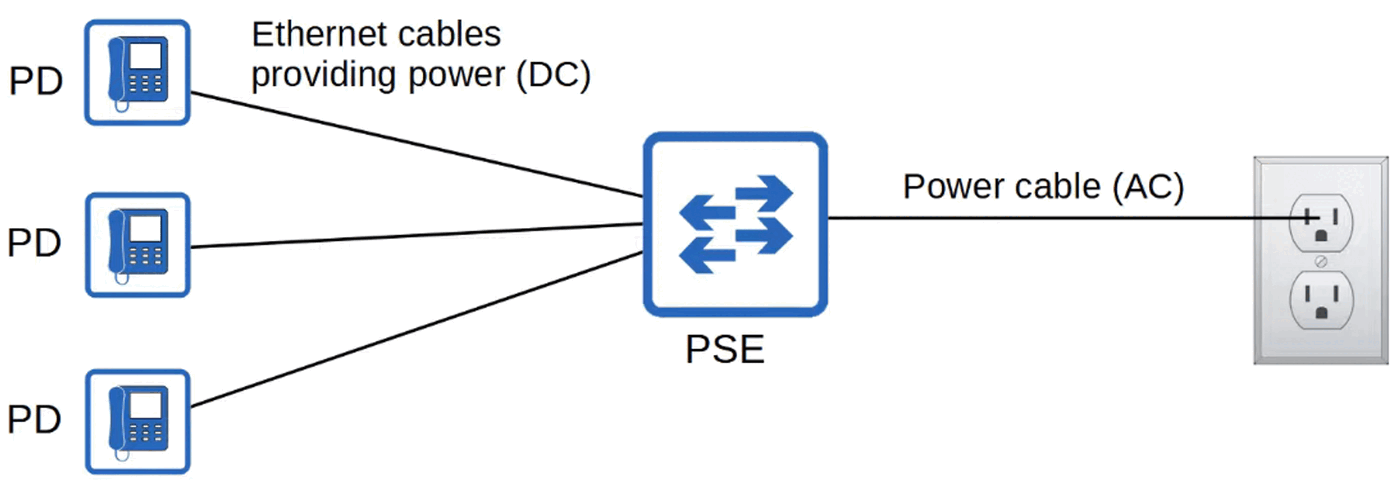
\includegraphics[keepaspectratio,alt={image}]{images/47-qos-voicelan/img-005.png}}
\end{figure}

\begin{itemize}
\tightlist
\item
  TOO much electrical current can damage electrical DEVICES
\item
  PoE has a process to determine if a CONNECTED DEVICE needs power and
  how much it needs.

  \begin{itemize}
  \tightlist
  \item
    When a DEVICE is connected to a PoE-Enabled PORT, the PSE (SWITCH)
    sends LOW POWER SIGNALS, monitors the response, and determines how
    much power the PD needs
  \item
    If the DEVICE needs POWER, the PSE supplies the POWER to allow the
    PD to boot
  \item
    The PSE continues to monitor the PD and SUPPLY the required amount
    of POWER (but not too much!)
  \end{itemize}
\item
  \emph{POWER POLICING} can be configured to prevent a PD from taking
  TOO much POWER

  \begin{itemize}
  \tightlist
  \item
    `power inline police' configures power policing with the default
    settings: disable the PORT and send a SYSLOG message if a PD draws
    too much power

    \begin{itemize}
    \tightlist
    \item
      Equivalent to `power inline police action err-disable'
    \item
      The INTERFACE will be put in an `error-disabled' state and can be
      re-enabled with `shutdown' followed by `no shutdown'
    \end{itemize}
  \end{itemize}

  \begin{figure}
  \centering
  \pandocbounded{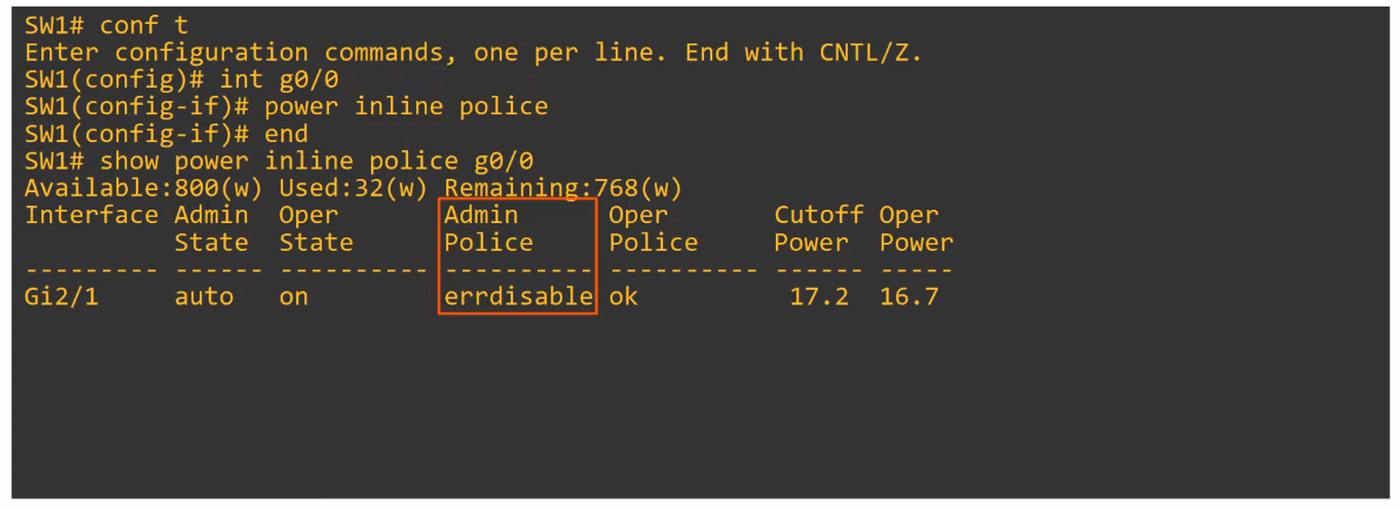
\includegraphics[keepaspectratio,alt={image}]{images/47-qos-voicelan/img-006.png}}
  \end{figure}

  \begin{itemize}
  \tightlist
  \item
    `power inline police action log' does NOT shut down the INTERFACE if
    the PD draws too much power. It WILL restart the INTERFACE and send
    a SYSLOG message
  \end{itemize}

  \begin{figure}
  \centering
  \pandocbounded{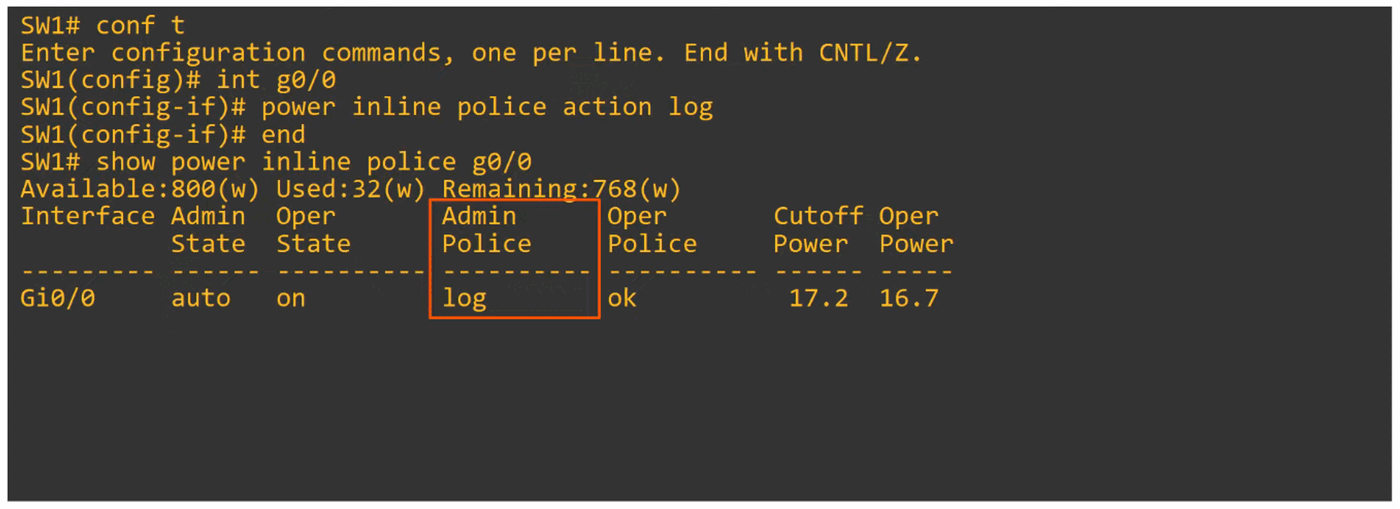
\includegraphics[keepaspectratio,alt={image}]{images/47-qos-voicelan/img-007.png}}
  \end{figure}

  \begin{figure}
  \centering
  \pandocbounded{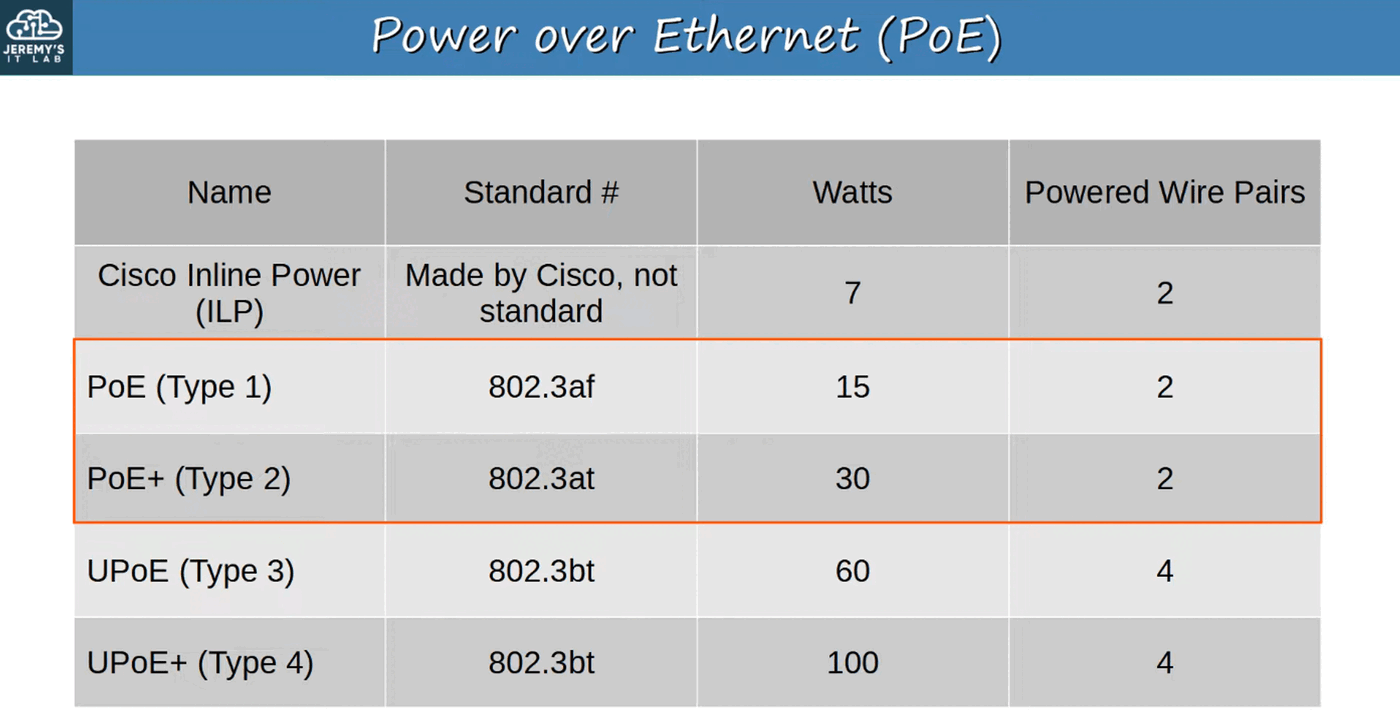
\includegraphics[keepaspectratio,alt={image}]{images/47-qos-voicelan/img-008.png}}
  \end{figure}
\end{itemize}

INTRO TO QUALITY OF SERVICE (QoS)

\begin{itemize}
\tightlist
\item
  VOICE traffic and DATA traffic used to use entirely separate NETWORKS

  \begin{itemize}
  \tightlist
  \item
    VOICE TRAFFIC used the PSTN
  \item
    DATA TRAFFIC used the IP NETWORK (Enterprise WAN, Internet, etc)
  \end{itemize}
\item
  QoS wasn't necessary as the different kinds of TRAFFIC didn't compete
  for BANDWIDTH
\end{itemize}

\begin{figure}
\centering
\pandocbounded{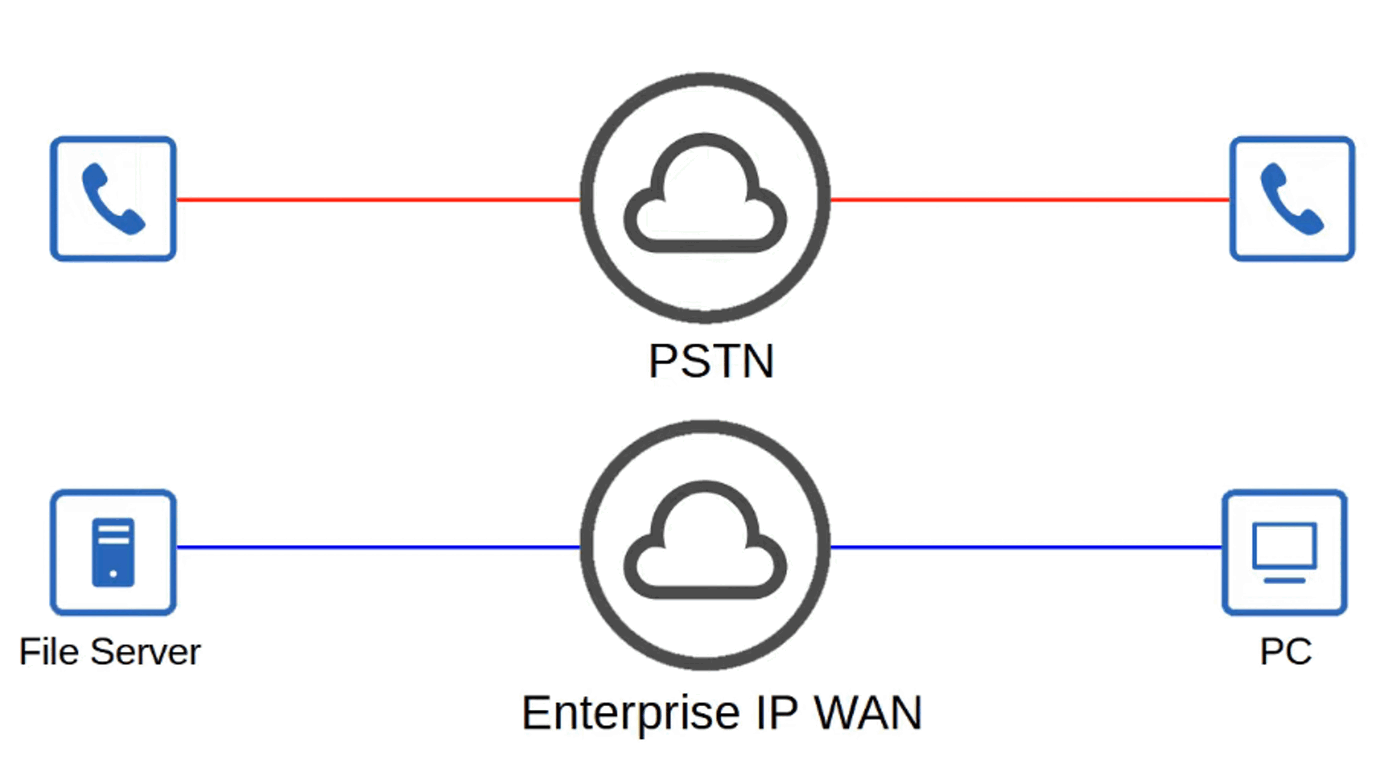
\includegraphics[keepaspectratio,alt={image}]{images/47-qos-voicelan/img-009.png}}
\end{figure}

\begin{itemize}
\tightlist
\item
  Modern NETWORKS are typically \emph{converged networks} in which IP
  PHONES, VIDEO TRAFFIC, REGULAR TRAFFIC, etc. all share the same IP
  NETWORK
\item
  This enables COST SAVINGS as well as more ADVANCED FEATURES for VOICE
  and VIDEO TRAFFIC (Example : Collaboration Software like Cisco WebEx,
  MS Teams, etc)
\item
  HOWEVER, the different kinds of TRAFFIC now have to compete for
  BANDWIDTH
\item
  \textbf{QoS} is a set of TOOLS used by NETWORK DEVICES to apply
  different TREATMENT to different PACKETS
\end{itemize}

\begin{figure}
\centering
\pandocbounded{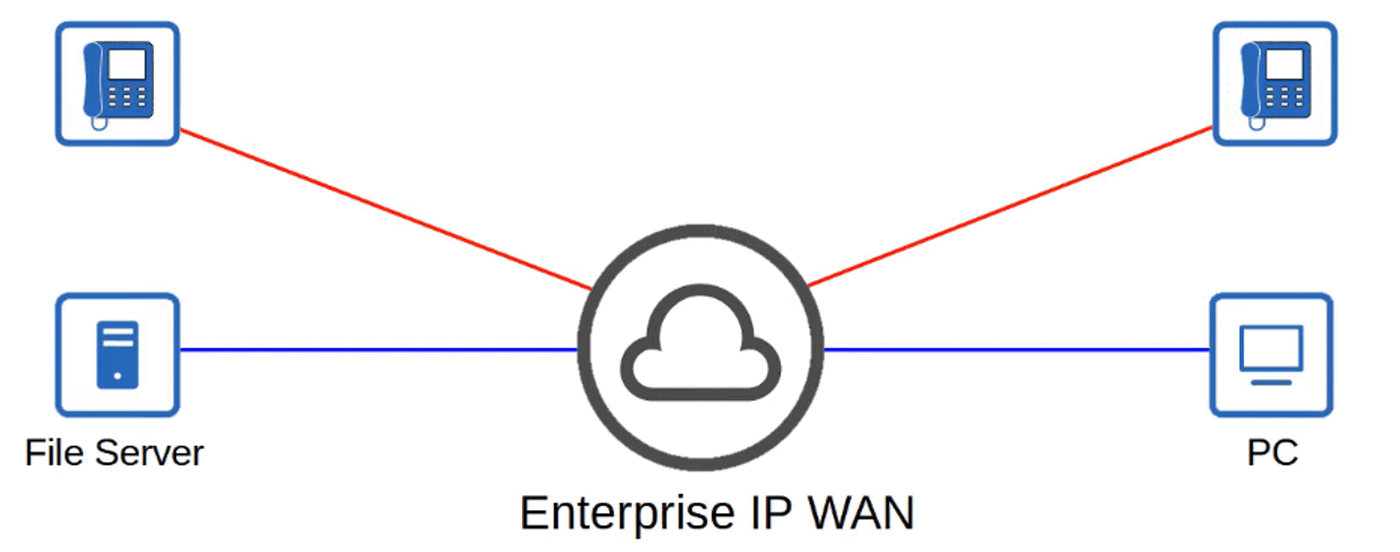
\includegraphics[keepaspectratio,alt={image}]{images/47-qos-voicelan/img-010.png}}
\end{figure}

QUALITY OF SERVICE (QoS)

\begin{itemize}
\tightlist
\item
  QoS is used to manage the following characteristics of NETWORK TRAFFIC

  \begin{itemize}
  \tightlist
  \item
    BANDWIDTH

    \begin{itemize}
    \tightlist
    \item
      Overall CAPACITY of the LINK (measured in \emph{bits per second})
    \item
      QoS TOOLS allow you to RESERVE a certain amount of a link's
      BANDWIDTH for specific kinds of traffic
    \end{itemize}
  \item
    DELAY

    \begin{itemize}
    \tightlist
    \item
      One-Way Delay = Time it takes traffic to go from SOURCE to
      DESTINATION
    \item
      Two-Way Delay = Time it takes traffic to go from SOURCE to
      DESTINATION and return
    \end{itemize}
  \end{itemize}
\end{itemize}

\begin{figure}
\centering
\pandocbounded{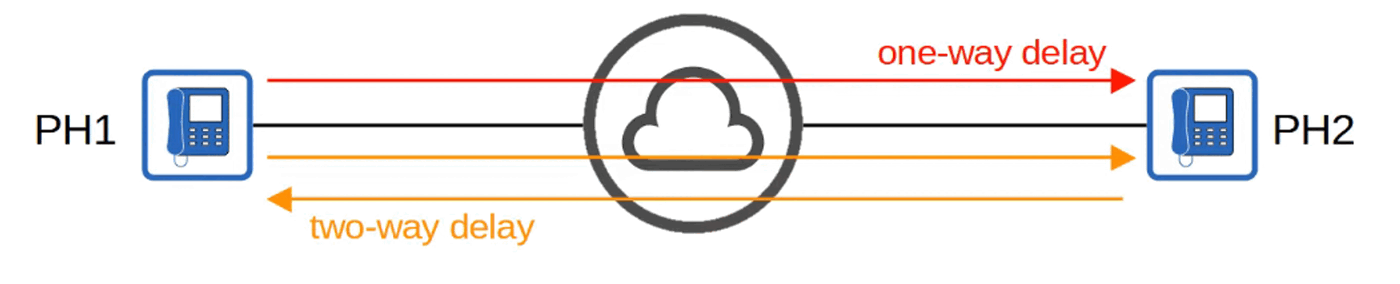
\includegraphics[keepaspectratio,alt={image}]{images/47-qos-voicelan/img-011.png}}
\end{figure}

\begin{lstlisting}
- JITTER
    - The variation in ONE-WAY DELAY between PACKETS SENT by the same APPLICATION
    - IP PHONES have a ‘jitter buffer’ to provide a FIXED DELAY to audio PACKETS
- LOSS
    - The % of PACKETS sent that DO NOT reach their DESTINATION
    - Can be caused by FAULTY CABLES
    - Can also be caused when a DEVICE’S PACKET QUEUES get full and the DEVICE starts discarding PACKETS
\end{lstlisting}

\begin{itemize}
\tightlist
\item
  The FOLLOWING STANDARDS are recommended for ACCEPTABLE INTERACTIVE
  AUDIO quality:

  \begin{itemize}
  \tightlist
  \item
    ONE-WAY DELAY : 150 milliseconds or less
  \item
    JITTER : 30 milliseconds or less
  \item
    LOSS : 1\% or less
  \end{itemize}
\item
  If these STANDARDS are not met, there could be a noticeable reduction
  in the QUALITY of the phone call
\end{itemize}

QoS QUEUING

\begin{itemize}
\tightlist
\item
  If a NETWORK DEVICE receives messages FASTER than it can FORWARD them
  out of the appropriate INTERFACE, the MESSAGES are placed in the QUEUE
\item
  By default, the QUEUED MESSAGES will be FORWARDED in a FIRST IN FIRST
  OUT (FIFO) manner

  \begin{itemize}
  \tightlist
  \item
    Message will be SENT in the ORDER they are RECEIVED
  \end{itemize}
\item
  If the QUEUE is FULL, new PACKETS will be DROPPED
\item
  The is called \emph{tail drop}
\end{itemize}

\begin{figure}
\centering
\pandocbounded{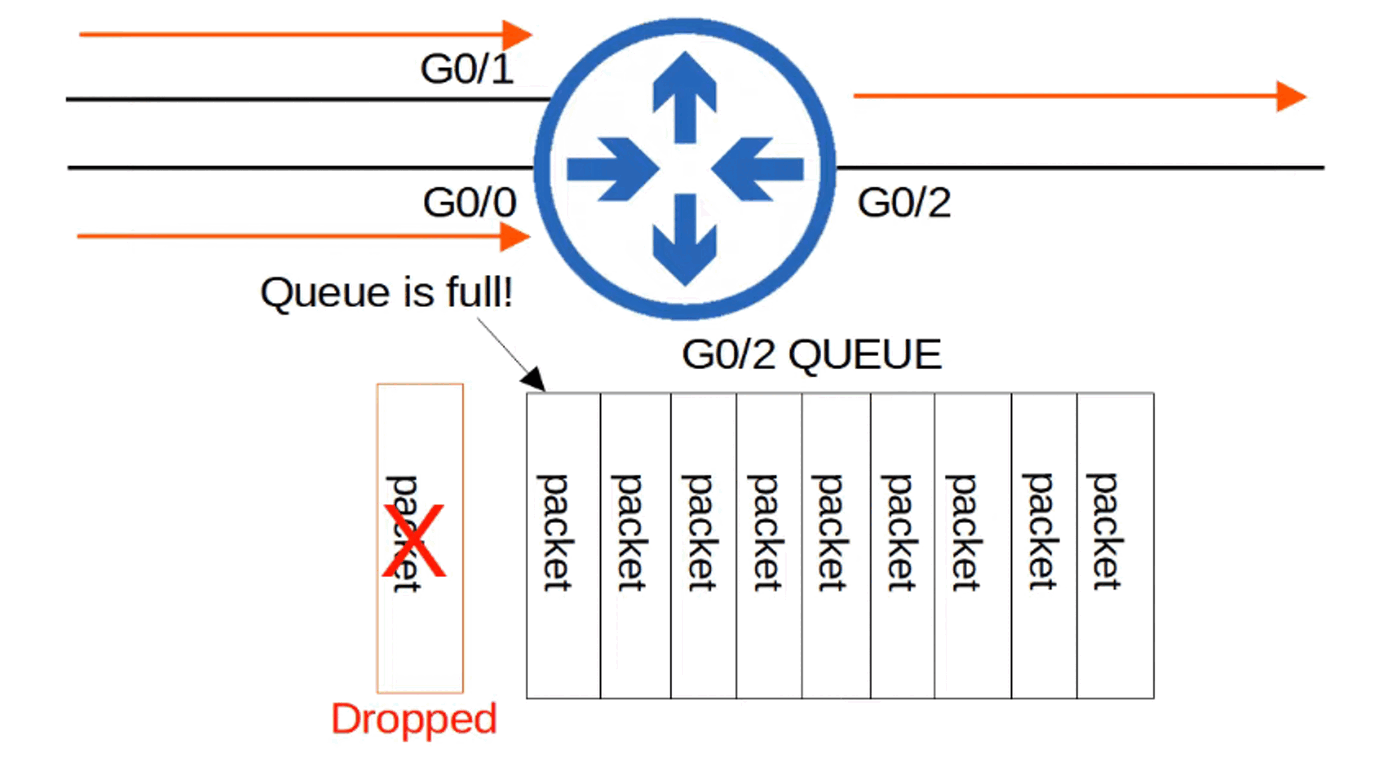
\includegraphics[keepaspectratio,alt={image}]{images/47-qos-voicelan/img-012.png}}
\end{figure}

\begin{itemize}
\tightlist
\item
  TAIL DROP is harmful because it can lead to TCP GLOBAL SYNCHRONIZATION
\end{itemize}

\begin{figure}
\centering
\pandocbounded{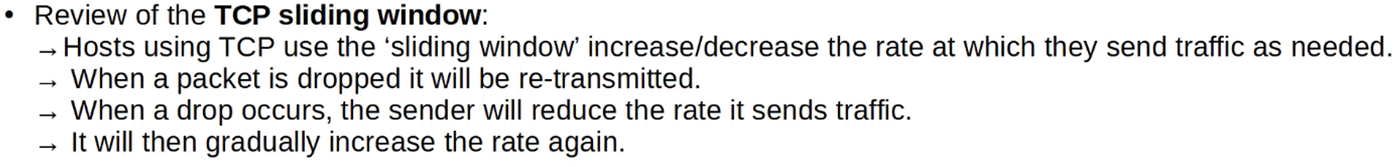
\includegraphics[keepaspectratio,alt={image}]{images/47-qos-voicelan/img-013.png}}
\end{figure}

\begin{itemize}
\tightlist
\item
  When the QUEUE fills UP and TAIL DROP occurs, ALL TCP HOSTS sending
  traffic will SLOW DOWN the rate at which they SEND TRAFFIC
\item
  They will ALL then INCREASE the RATE at which they send TRAFFIC, which
  rapidly leads to MORE CONGESTION, dropped PACKETS, and the process
  REPEATS\ldots{}
\end{itemize}

\begin{figure}
\centering
\pandocbounded{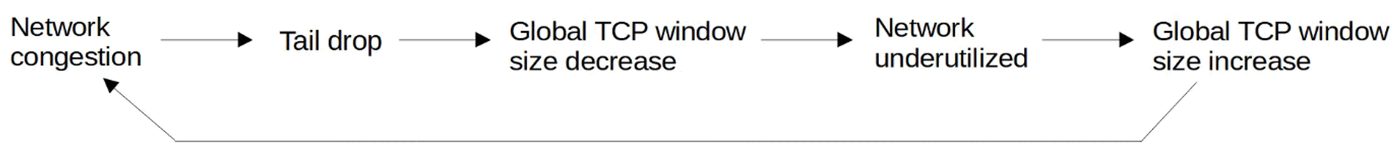
\includegraphics[keepaspectratio,alt={image}]{images/47-qos-voicelan/img-014.png}}
\end{figure}

\begin{itemize}
\item
  A SOLUTION to prevent TAIL DROP and TCP GLOBAL SYNCHRONIZATION is
  RANDOM EARLY DETECTION (RED)
\item
  When the amount of TRAFFIC in the QUEUE reaches a certain THRESHOLD,
  the DEVICE will start RANDOMLY dropping PACKETS from select TCP FLOWS
\item
  Those TCP FLOWS that dropped PACKETS will reduce the RATE at which
  TRAFFIC is sent, but you will avoid TCP GLOBAL SYNCHRONIZATION, in
  which ALL TCP FLOWS reduce and then increase the rate of transmission
  at the same time, in waves.
\item
  In STANDARD RED, all kinds of TRAFFIC are treated the SAME
\item
  WEIGHTED RANDOM EARLY DETECTION (WRED) - an improved version of RED,
  allows you control which PACKETS are dropped depending on the TRAFFIC
  CLASS
\end{itemize}

** TRAFFIC CLASSES and details about how QoS works will be covered in
DAY 47 **
